\documentclass[10pt,a4paper]{article}
\usepackage[utf8]{inputenc}
\usepackage[german]{babel}
\usepackage{mathrsfs}
\usepackage{amsmath}
\usepackage{amsfonts}
\usepackage{amssymb}
\usepackage{amsthm}
\usepackage[left=2cm,right=2cm,top=2cm,bottom=2cm]{geometry}
\usepackage{graphicx}
\usepackage{float}

\begin{document}

\section{Aufgabe 5.1}

Nein. Wenn die SampleRTT nicht konstant ist, hat das TimeoutInterval noch einen
weiteren Summanden, der von der Schwankung der SampleRTT abhängt.

\section{Aufgabe 5.2}

\subsection{Teil 1}

Falsch. Wenn für eine bestimmte Zeit keine Datenpakete für Host A auf Host B
produziert wurden, schickt Host B einfach extra ACKs.

\subsection{Teil 2}

Falsch. Das RcvWindow ist immer so groß, wie der Empfänger noch Platz hat.

\subsection{Teil 3}

Richtig.

\section{Aufgabe 5.3}

$\frac{R}{2}$, wenn beide Hosts an Ziele mit identischer RTT senden. Andernfalls wird es nur gegen $\frac{R}{2}$ konvergieren.

\section{Aufgabe 5.4}

\subsection{Teil 1}

Das erste Segment beginnt mit Byte Nr. 80 und das zweite mit Byte Nr. 120. Das
erste Paket enthält also $120 - 80 = 40$ Byte.

\subsection{Teil 2}

Bei einem einzelnen Verlust, wird bei jedem nachfolgendem Paket mit der
Sequenznummer des noch fehlenden Pakets geantwortet. In diesem Fall sendet der
Empfänger also ein $ACK=80$.

\section{Aufgabe 5.5}

\subsection{Teil 1}

Die Portnummern ändern sich nicht, nur die Sequenznummer wird angepasst. Also
ist die Quellportnummer 503, die Zielportnummer 80 und die Sequenznummer
$249 + 40 = 289$.

\subsection{Teil 2}

Quellport $80$, Zielport $503$, ACK $289$.

\subsection{Teil 3}

$249$

\subsection{Teil 4}

\begin{figure}[H]
  \centering
  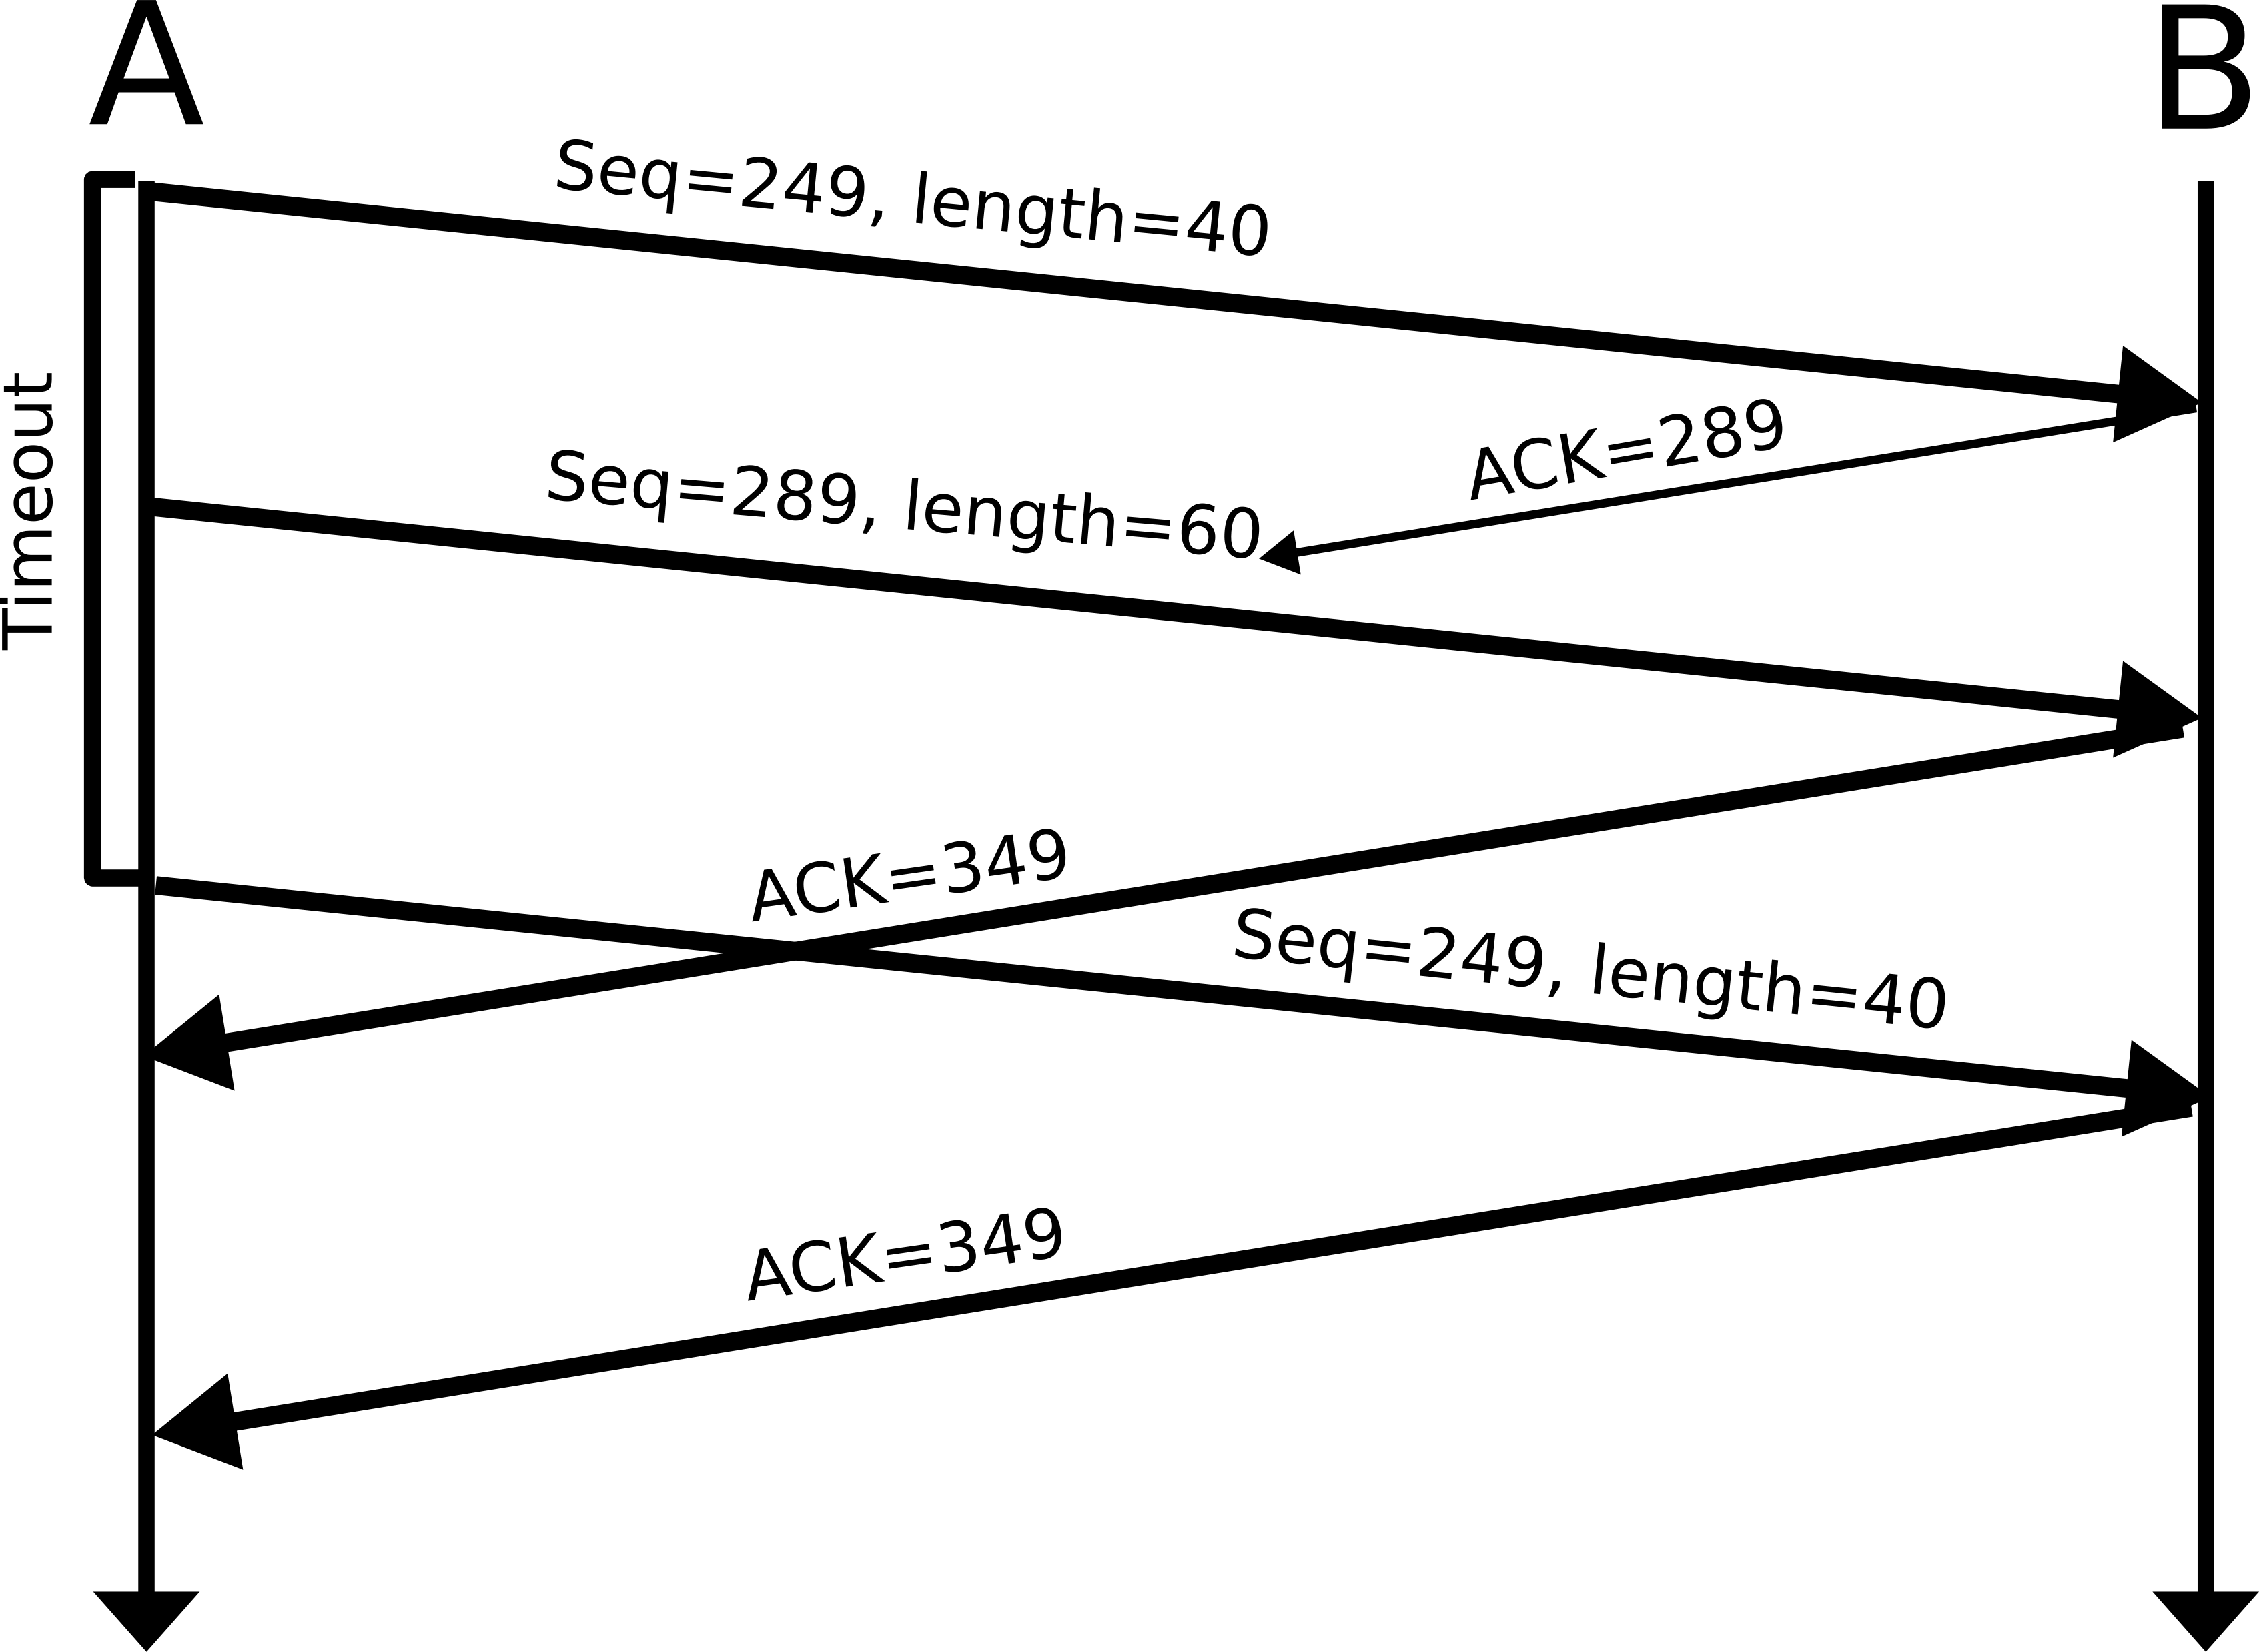
\includegraphics[width=250pt]{5_5_4}
\end{figure}

\section{Aufgabe 5.6}

\begin{figure}[H]
  \centering
  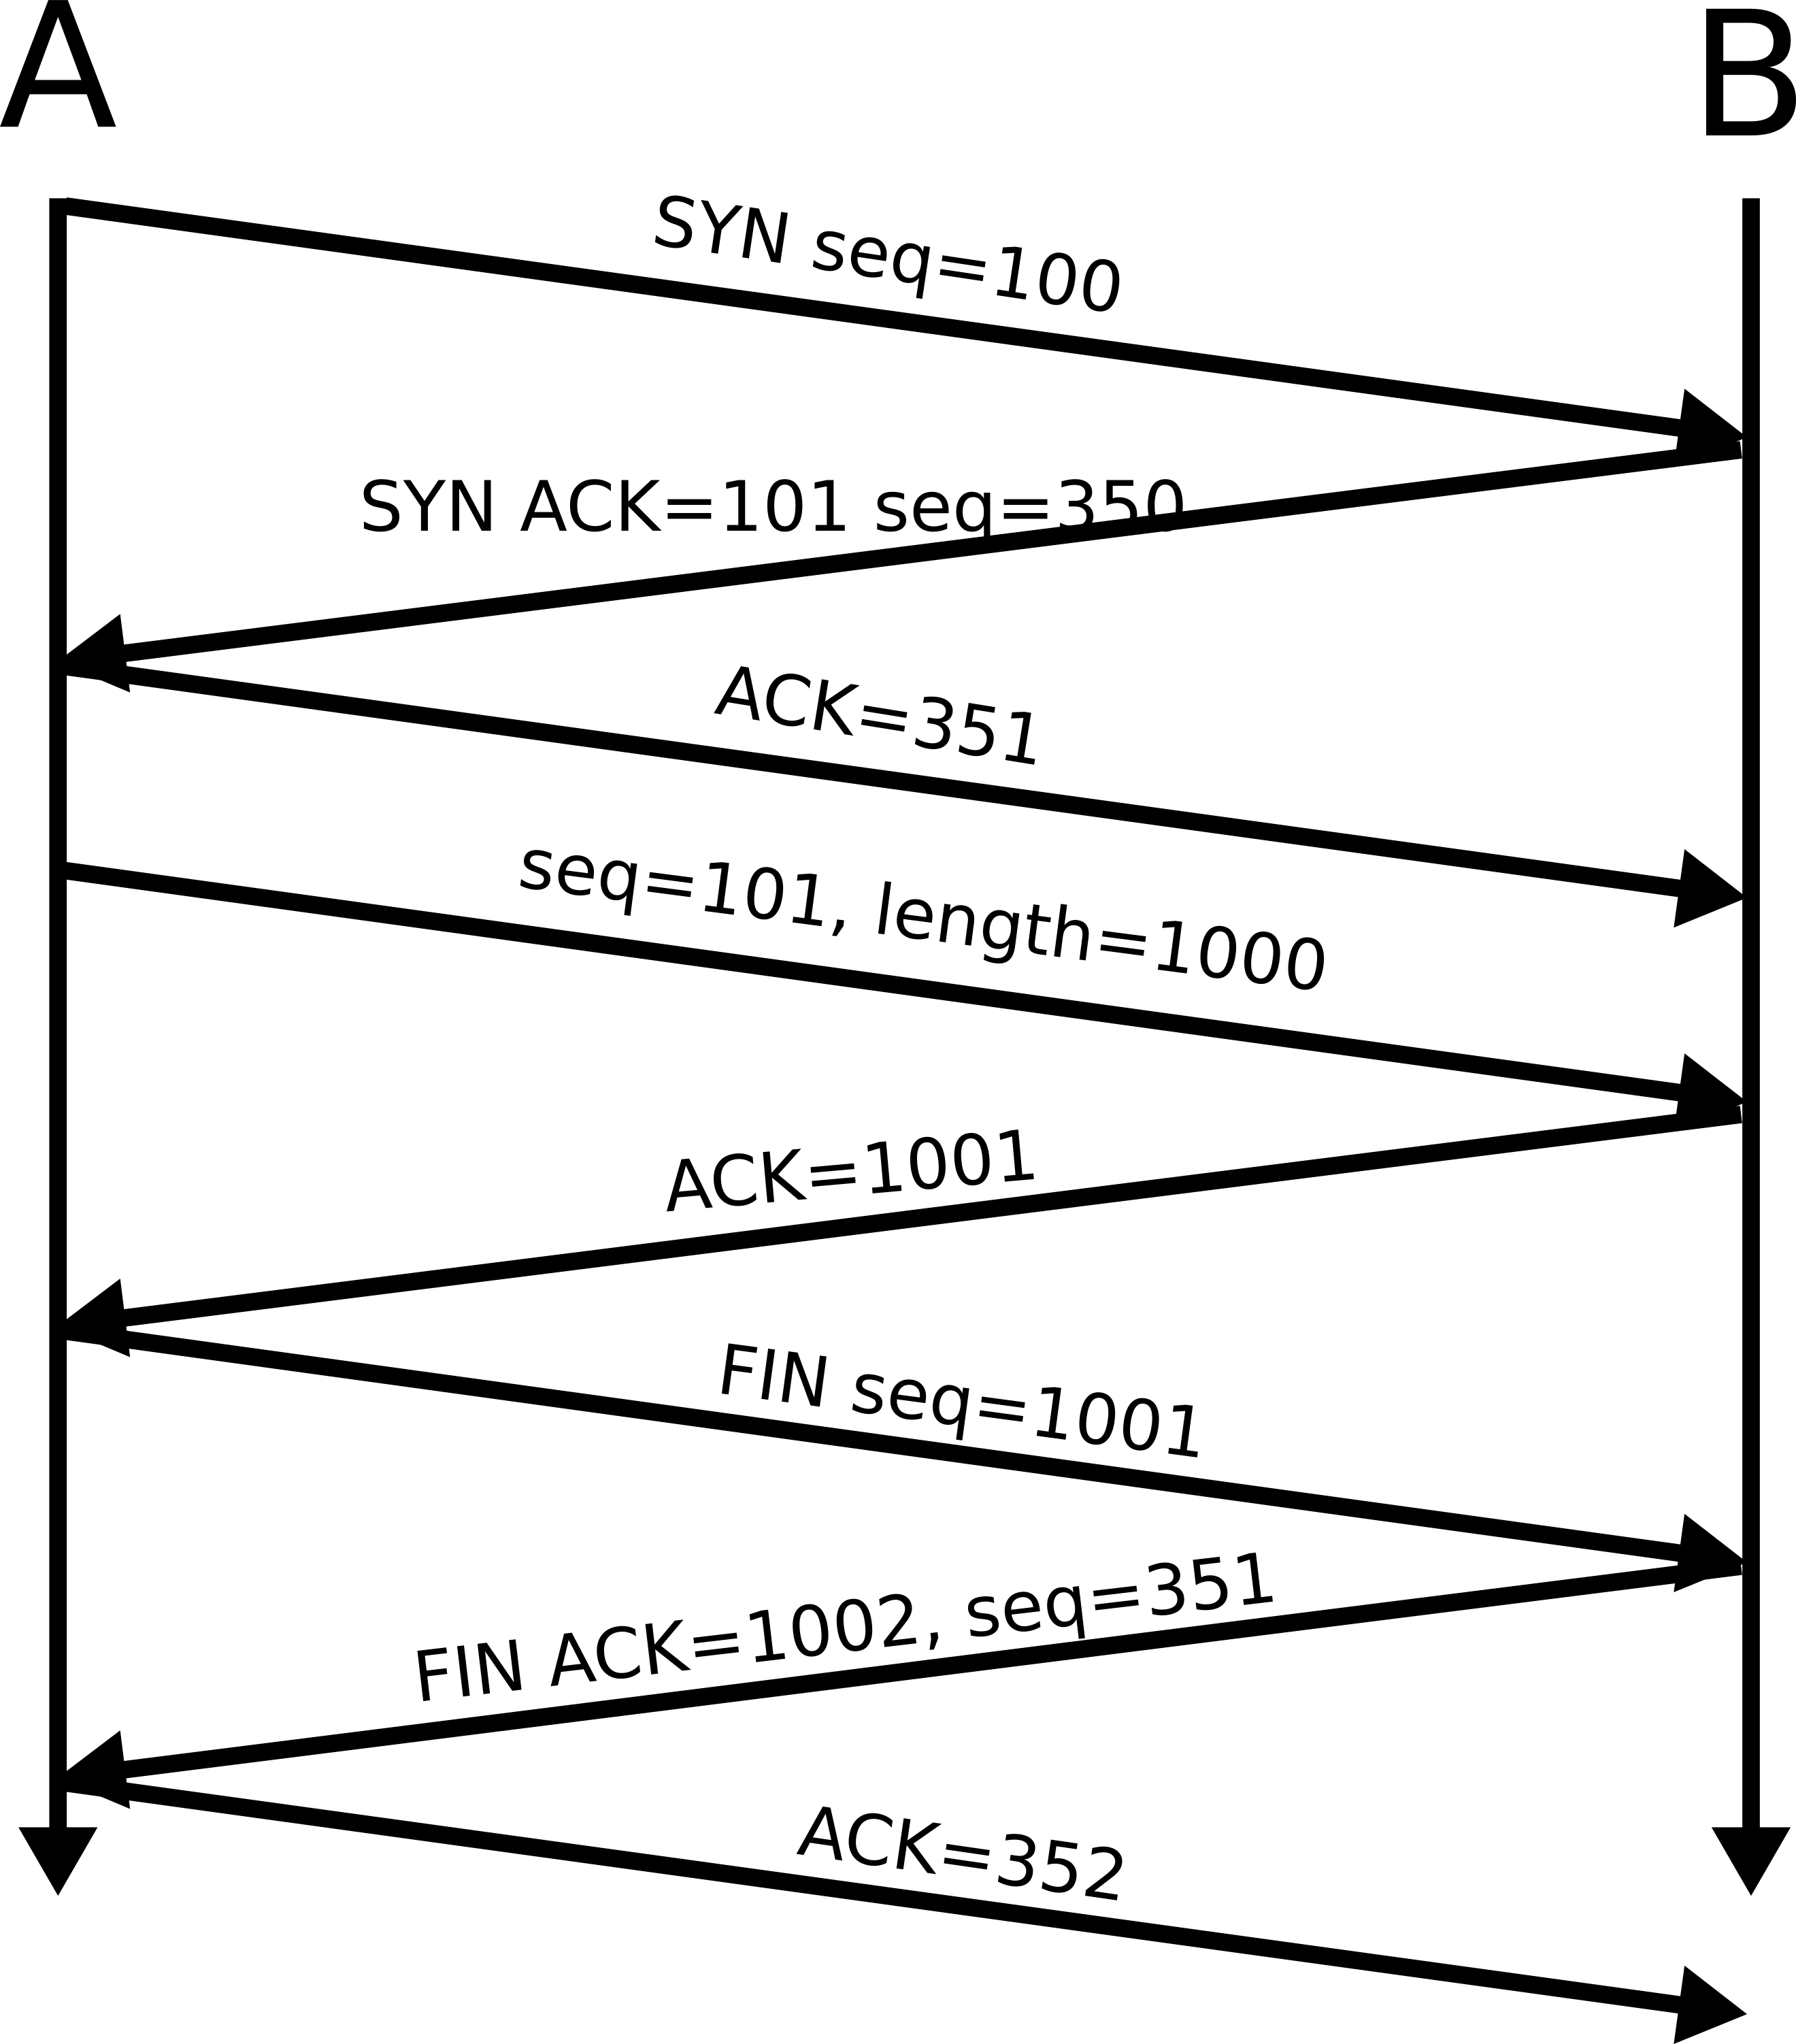
\includegraphics[width=250pt]{5_6}
\end{figure}

\section{Aufgabe 5.7}

RFC2001 sagt, dass 3 doppelte ACKS ein klares Zeichen dafür sind, dass ein Paket
verloren gegangen ist. Weniger als 3 Dopplungen können auch oft dadurch
entstehen, dass Pakete nur in falscher Reihenfolge ausgeliefert wurden, aber
doch alle angekommen sind.

\section{Aufgabe 5.8}

\subsection{Teil 1}

0-5, 21-25

\subsection{Teil 2}

5-13, 14-20

\subsection{Teil 3}

13-14

\subsection{Teil 4}

20-21

\subsection{Teil 5}

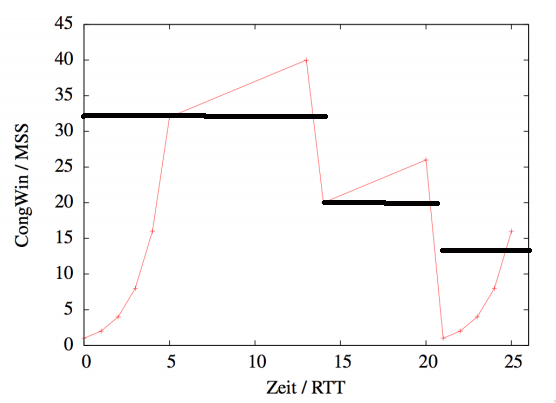
\includegraphics[width=250pt]{5_8_5.png}

\end{document}